\documentclass[11pt,compress,t,notes=noshow, xcolor=table]{beamer}
\usepackage[]{graphicx}\usepackage[]{color}
% maxwidth is the original width if it is less than linewidth
% otherwise use linewidth (to make sure the graphics do not exceed the margin)
\makeatletter
\def\maxwidth{ %
  \ifdim\Gin@nat@width>\linewidth
    \linewidth
  \else
    \Gin@nat@width
  \fi
}
\makeatother

\definecolor{fgcolor}{rgb}{0.345, 0.345, 0.345}
\newcommand{\hlnum}[1]{\textcolor[rgb]{0.686,0.059,0.569}{#1}}%
\newcommand{\hlstr}[1]{\textcolor[rgb]{0.192,0.494,0.8}{#1}}%
\newcommand{\hlcom}[1]{\textcolor[rgb]{0.678,0.584,0.686}{\textit{#1}}}%
\newcommand{\hlopt}[1]{\textcolor[rgb]{0,0,0}{#1}}%
\newcommand{\hlstd}[1]{\textcolor[rgb]{0.345,0.345,0.345}{#1}}%
\newcommand{\hlkwa}[1]{\textcolor[rgb]{0.161,0.373,0.58}{\textbf{#1}}}%
\newcommand{\hlkwb}[1]{\textcolor[rgb]{0.69,0.353,0.396}{#1}}%
\newcommand{\hlkwc}[1]{\textcolor[rgb]{0.333,0.667,0.333}{#1}}%
\newcommand{\hlkwd}[1]{\textcolor[rgb]{0.737,0.353,0.396}{\textbf{#1}}}%
\let\hlipl\hlkwb

\usepackage{framed}
\makeatletter
\newenvironment{kframe}{%
 \def\at@end@of@kframe{}%
 \ifinner\ifhmode%
  \def\at@end@of@kframe{\end{minipage}}%
  \begin{minipage}{\columnwidth}%
 \fi\fi%
 \def\FrameCommand##1{\hskip\@totalleftmargin \hskip-\fboxsep
 \colorbox{shadecolor}{##1}\hskip-\fboxsep
     % There is no \\@totalrightmargin, so:
     \hskip-\linewidth \hskip-\@totalleftmargin \hskip\columnwidth}%
 \MakeFramed {\advance\hsize-\width
   \@totalleftmargin\z@ \linewidth\hsize
   \@setminipage}}%
 {\par\unskip\endMakeFramed%
 \at@end@of@kframe}
\makeatother

\definecolor{shadecolor}{rgb}{.97, .97, .97}
\definecolor{messagecolor}{rgb}{0, 0, 0}
\definecolor{warningcolor}{rgb}{1, 0, 1}
\definecolor{errorcolor}{rgb}{1, 0, 0}
\newenvironment{knitrout}{}{} % an empty environment to be redefined in TeX

\usepackage{alltt}
\newcommand{\SweaveOpts}[1]{}  % do not interfere with LaTeX
\newcommand{\SweaveInput}[1]{} % because they are not real TeX commands
\newcommand{\Sexpr}[1]{}       % will only be parsed by R



\usepackage[english]{babel}
\usepackage[utf8]{inputenc}

\usepackage{dsfont}
\usepackage{verbatim}
\usepackage{amsmath}
\usepackage{amsfonts}
\usepackage{bm}
\usepackage{csquotes}
\usepackage{multirow}
\usepackage{longtable}
\usepackage{booktabs}
\usepackage{enumerate}
\usepackage[absolute,overlay]{textpos}
\usepackage{psfrag}
\usepackage{algorithm}
\usepackage{algpseudocode}
\usepackage{eqnarray}
\usepackage{arydshln}
\usepackage{tabularx}
\usepackage{placeins}
\usepackage{tikz}
\usepackage{setspace}
\usepackage{colortbl}
\usepackage{mathtools}
\usepackage{wrapfig}
\usepackage{bm}
\usetikzlibrary{shapes,arrows,automata,positioning,calc,chains,trees, shadows}
\tikzset{
  %Define standard arrow tip
  >=stealth',
  %Define style for boxes
  punkt/.style={
    rectangle,
    rounded corners,
    draw=black, very thick,
    text width=6.5em,
    minimum height=2em,
    text centered},
  % Define arrow style
  pil/.style={
    ->,
    thick,
    shorten <=2pt,
    shorten >=2pt,}
}
\usepackage{subfig}


% Defines macros and environments
\usepackage{bbm}
% basic latex stuff
\newcommand{\pkg}[1]{{\fontseries{b}\selectfont #1}} %fontstyle for R packages
\newcommand{\lz}{\vspace{0.5cm}} %vertical space
\newcommand{\dlz}{\vspace{1cm}} %double vertical space
\newcommand{\oneliner}[1] % Oneliner for important statements
{\begin{block}{}\begin{center}\begin{Large}#1\end{Large}\end{center}\end{block}}


%new environments
\newenvironment{vbframe}  %frame with breaks and verbatim
{
 \begin{frame}[containsverbatim,allowframebreaks]
}
{
\end{frame}
}

\newenvironment{vframe}  %frame with verbatim without breaks (to avoid numbering one slided frames)
{
 \begin{frame}[containsverbatim]
}
{
\end{frame}
}

\newenvironment{blocki}[1]   % itemize block
{
 \begin{block}{#1}\begin{itemize}
}
{
\end{itemize}\end{block}
}

\newenvironment{fragileframe}[2]{  %fragile frame with framebreaks
\begin{frame}[allowframebreaks, fragile, environment = fragileframe]
\frametitle{#1}
#2}
{\end{frame}}


\newcommand{\myframe}[2]{  %short for frame with framebreaks
\begin{frame}[allowframebreaks]
\frametitle{#1}
#2
\end{frame}}

\newcommand{\remark}[1]{
  \textbf{Remark:} #1
}


\newenvironment{deleteframe}
{
\begingroup
\usebackgroundtemplate{
\includegraphics[width=\paperwidth,height=\paperheight]{../style/color/red.png}}
 \begin{frame}
}
{
\end{frame}
\endgroup
}
\newenvironment{simplifyframe}
{
\begingroup
\usebackgroundtemplate{
\includegraphics[width=\paperwidth,height=\paperheight]{../style/color/yellow.png}}
 \begin{frame}
}
{
\end{frame}
\endgroup
}\newenvironment{draftframe}
{
\begingroup
\usebackgroundtemplate{
\includegraphics[width=\paperwidth,height=\paperheight]{../style/color/green.jpg}}
 \begin{frame}
}
{
\end{frame}
\endgroup
}
% https://tex.stackexchange.com/a/261480: textcolor that works in mathmode
\makeatletter
\renewcommand*{\@textcolor}[3]{%
  \protect\leavevmode
  \begingroup
    \color#1{#2}#3%
  \endgroup
}
\makeatother

% \usepackage{bbm}
% basic latex stuff
\newcommand{\pkg}[1]{{\fontseries{b}\selectfont #1}} %fontstyle for R packages
\newcommand{\lz}{\vspace{0.5cm}} %vertical space
\newcommand{\dlz}{\vspace{1cm}} %double vertical space
\newcommand{\oneliner}[1] % Oneliner for important statements
{\begin{block}{}\begin{center}\begin{Large}#1\end{Large}\end{center}\end{block}}


%new environments
\newenvironment{vbframe}  %frame with breaks and verbatim
{
 \begin{frame}[containsverbatim,allowframebreaks]
}
{
\end{frame}
}

\newenvironment{vframe}  %frame with verbatim without breaks (to avoid numbering one slided frames)
{
 \begin{frame}[containsverbatim]
}
{
\end{frame}
}

\newenvironment{blocki}[1]   % itemize block
{
 \begin{block}{#1}\begin{itemize}
}
{
\end{itemize}\end{block}
}

\newenvironment{fragileframe}[2]{  %fragile frame with framebreaks
\begin{frame}[allowframebreaks, fragile, environment = fragileframe]
\frametitle{#1}
#2}
{\end{frame}}


\newcommand{\myframe}[2]{  %short for frame with framebreaks
\begin{frame}[allowframebreaks]
\frametitle{#1}
#2
\end{frame}}

\newcommand{\remark}[1]{
  \textbf{Remark:} #1
}


\newenvironment{deleteframe}
{
\begingroup
\usebackgroundtemplate{
\includegraphics[width=\paperwidth,height=\paperheight]{../style/color/red.png}}
 \begin{frame}
}
{
\end{frame}
\endgroup
}
\newenvironment{simplifyframe}
{
\begingroup
\usebackgroundtemplate{
\includegraphics[width=\paperwidth,height=\paperheight]{../style/color/yellow.png}}
 \begin{frame}
}
{
\end{frame}
\endgroup
}\newenvironment{draftframe}
{
\begingroup
\usebackgroundtemplate{
\includegraphics[width=\paperwidth,height=\paperheight]{../style/color/green.jpg}}
 \begin{frame}
}
{
\end{frame}
\endgroup
}
% https://tex.stackexchange.com/a/261480: textcolor that works in mathmode
\makeatletter
\renewcommand*{\@textcolor}[3]{%
  \protect\leavevmode
  \begingroup
    \color#1{#2}#3%
  \endgroup
}
\makeatother


%\usetheme{lmu-lecture}
\newcommand{\titlefigure}{figure/cart_dis_1}
\newcommand{\learninggoals}{
\item Understand advantages and disadvantages of CART
\item Know how CART can be expressed in terms of hypothesis space, risk and optimization}
\usepackage{../../style/lmu-lecture}

\let\code=\texttt
\let\proglang=\textsf

\setkeys{Gin}{width=0.9\textwidth}

\title{Introduction to Machine Learning}
% \author{Bernd Bischl, Christoph Molnar, Daniel Schalk, Fabian Scheipl}
\institute{\href{https://compstat-lmu.github.io/lecture_i2ml/}{compstat-lmu.github.io/lecture\_i2ml}}
\date{}

\setbeamertemplate{frametitle}{\expandafter\uppercase\expandafter\insertframetitle}



\begin{document}
% Introduction to Machine Learning
% Day 4

% Set style/preamble.Rnw as parent.


% Load all R packages and set up knitr

% This file loads R packages, configures knitr options and sets preamble.Rnw as parent file
% IF YOU MODIFY THIS, PLZ ALSO MODIFY setup.Rmd ACCORDINGLY...








% Defines macros and environments
\input{../../latex-math/basic-ml.tex}

%! includes: cart-stoppingpruning

\lecturechapter{CART: Advantages \& Disadvantages}
\lecture{Introduction to Machine Learning}

\sloppy

\begin{vbframe}{Advantages}
  \begin{itemize}
    \item Fairly easy to understand, interpret and visualize.
    \item Not much preprocessing required:
    \begin{itemize}
      \item automatic handling of non-numerical features
      \item automatic handling of missing values via surrogate splits
      \item no problems with outliers in features
      \item monotone transformations of features change nothing so scaling of features is irrelevant
    \end{itemize}
    \item Interaction effects between features are easily possible, even of higher orders
    \item Can model discontinuities and non-linearities (but see "disadvantages")
    
    \framebreak
    
    \item Performs automatic feature selection
    \item Quite fast, scales well with larger data
    \item Flexibility through definition of custom split criteria or leaf-node prediction rules: clustering trees, semi-supervised trees, density estimation, etc.
  \end{itemize}
\end{vbframe}

\begin{vbframe}{Disadvantage: Linear Dependencies}
\begin{knitrout}\scriptsize
\definecolor{shadecolor}{rgb}{0.969, 0.969, 0.969}\color{fgcolor}

{\centering 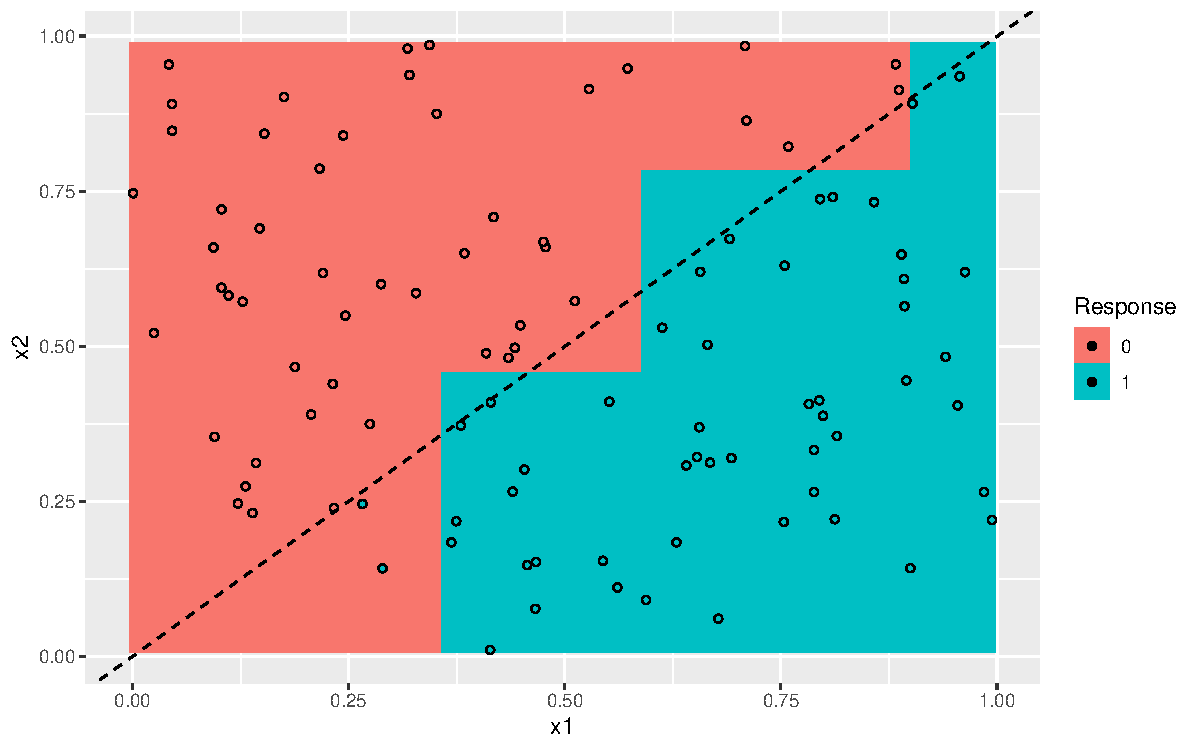
\includegraphics[width=0.95\textwidth]{figure/cart_dis_1} 

}



\end{knitrout}
Linear dependencies must be modeled over several splits. Logistic regression would model this easily.
\end{vbframe}

\begin{vbframe}{Disadvantage: Smooth functions}
\begin{knitrout}\scriptsize
\definecolor{shadecolor}{rgb}{0.969, 0.969, 0.969}\color{fgcolor}

{\centering 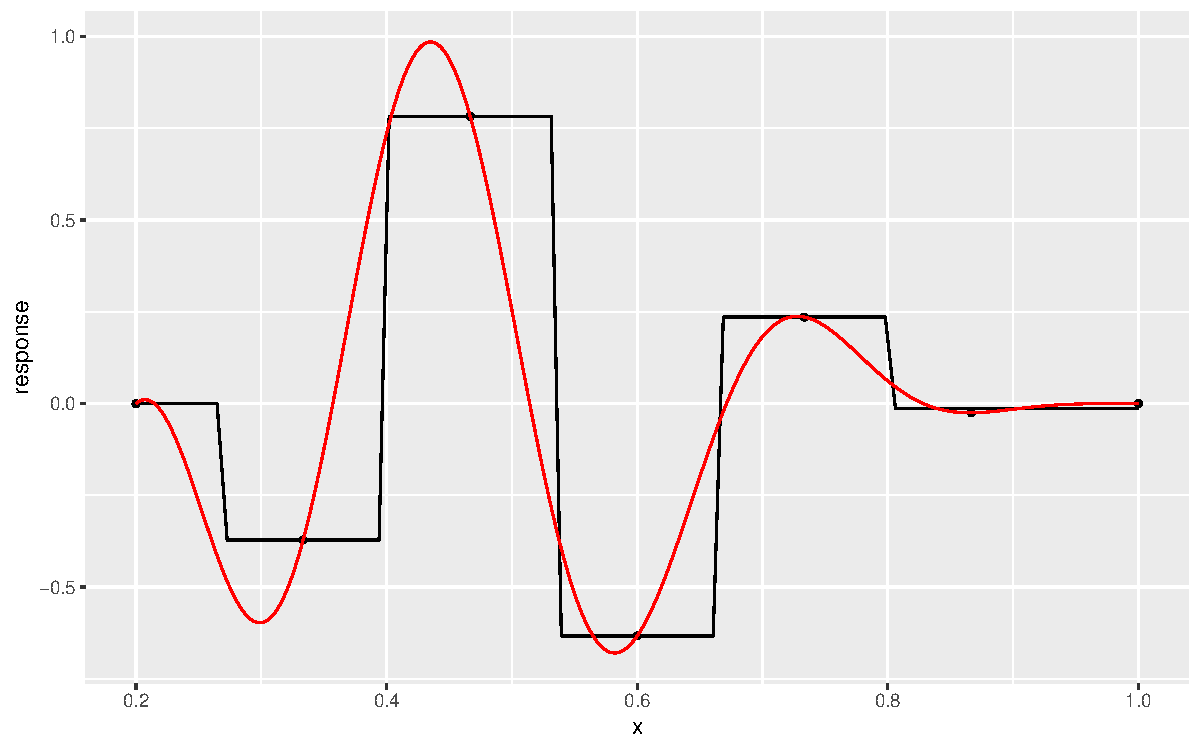
\includegraphics[width=0.95\textwidth]{figure/cart_dis_2} 

}



\end{knitrout}
Prediction functions of trees are never smooth as they are always step functions.
\end{vbframe}

% \begin{vbframe}{Disadvantage: Instability}
% \begin{itemize}
% \item High instability (variance) of the trees:
% \item Small changes in the data could lead to completely different splits / trees
% \item This leads to a) less trust in interpretability b) is a reason why prediction error of trees is usually not best, compared with other models
% \end{itemize}

% \framebreak

% High instability of trees will be demonstrated using the Wisconsin Breast Cancer data set.
% It has 699 observations on 9 features and one target class with values \enquote{benign} and \enquote{malignant}.

% \begin{table}
% \begin{tabular}{ll}
% Feature name & Explanation\\
% \hline
% \code{Cl.thickness} & Clump Thickness\\
% \code{Cell.size} & Uniformity of Cell Size\\
% \code{Cell.shape} & Uniformity of Cell Shape\\
% \code{Marg.adhesion} & Marginal Adhesion\\
% \code{Epith.c.size} & Single Epithelial Cell Size\\
% \code{Bare.nuclei} & Bare Nuclei\\
% \code{Bl.cromatin} & Bland Chromatin\\
% \code{Normal.nucleoli} & Normal Nucleoli\\
% \code{Mitoses} & Mitoses\\
% \end{tabular}
% \end{table}

% \framebreak

% Tree fitted on complete Wisconsin Breast Cancer data
% <<results='hide', fig.height=5>>=
% # BB: i am using the BC dataset directly from mlbench
% # and convert features, see issue in i2ml nr 277
% library(mlbench)
% data(BreastCancer)
% d = BreastCancer
% d$Id = NULL
% for (i in 1:9)
%   d[,i] = as.integer(d[,i])
% print(str(d))
% lrn = makeLearner("classif.rpart")
% task1 = makeClassifTask(data = d, target = "Class")
% mod1 = train(lrn, task1)
% d2 = d[-13, ]
% task2 = makeClassifTask(data = d2, target = "Class")
% mod2 = train(lrn, task2)
% fancyRpartPlot(mod1$learner.model, sub = "")
% @
% \framebreak

% Tree fitted on Wisconsin Breast Cancer data without observation 13
% <<results='hide', fig.height=5>>=
% fancyRpartPlot(mod2$learner.model, sub = "")
% @
% \end{vbframe}

\begin{vbframe}{Disadvantages}
\begin{itemize}
\item Empirically not the best predictor: Combine with bagging (forest) or boosting!
\item High instability (variance) of the trees.
  Small changes in the training data can lead to completely different trees. This leads to reduced trust in interpretation and is a reason why prediction errors of trees are usually not the best.
\item In regression: Trees define piecewise constant functions, so trees often do not extrapolate well.
\end{itemize}
\end{vbframe}

\begin{vbframe}{Further tree methodologies}

\begin{itemize}
\item AID (Sonquist and Morgan, 1964)
\item CHAID (Kass, 1980)
\item CART (Breiman et al., 1984)
\item C4.5 (Quinlan, 1993)
\item Unbiased Recursive Partitioning (Hothorn et al., 2006)
\end{itemize}

\end{vbframe}

\begin{vbframe}{CART: Synopsis}
\textbf{Hypothesis Space:}\\
CART models are step functions over a rectangular partition of $\Xspace$.\\
Their maximal complexity is controlled by the stopping criteria and the pruning method.

\lz

\textbf{Risk:}\\
Trees can use any kind of loss function for regression or classification.

\lz

\textbf{Optimization:}\\
Exhaustive search over all possible splits in each node to minimize the empirical risk in the child nodes.\\

{\small
Most literature on CARTs based on \enquote{impurity reduction} which is mathematically equivalent to empirical risk minimization:\\
Gini impurity $\cong$ Brier Score loss,\\ entropy impurity $\cong$  
Bernoulli loss,\\ variance impurity $\cong$ L2 loss.}

\end{vbframe}

\endlecture
\end{document}
